\chapter{DYNAMIC WIDTHS OF ICE-I$_\mathrm{h}$ / WATER INTERFACES}\label{chap:Dyn}

The spatially-resolved orientational time correlation function,
\begin{equation}\label{C(t)1}
  C_{2}(z,t)=\langle P_{2}(\mathbf{u}_i(0)\cdot \mathbf{u}_i(t))
  \delta(z_i(0) - z) \rangle,
\end{equation}
provides local information about the decorrelation of molecular
orientations in time. Here, $P_{2}$ is the second-order Legendre
polynomial, and $\mathbf{u}_i$ is the molecular unit vector that bisects
the HOH angle of molecule $i$. The angle brackets indicate an average
over all the water molecules and time origins, and the delta function
restricts the average to specific regions in the $z$-dimension. 

In the ice crystal, decay of $C_2(z,t)$ is incomplete, while in the
liquid, correlation times are typically measured in ps. Observing the
spatial transition between the decay regimes can define a dynamic
measure of the interfacial width. To determine dynamic widths of the
interfaces under shear, each of the systems were divided into bins
along the $z$ axis ($\approx$ 1 \AA\ wide) and $C_2(z,t)$ was computed
using only those molecules that were in the bin at the initial
time. For each ice / water interface investigated, the following 0.5
ns simulations were computed: quiescent simulations (where no thermal
or momentum gradient was present), simulations with only a thermal
gradient present, and simulations where both thermal and momentum
gradients were present. During these simulations, the positions and
orientations of each molecule were recorded every 100 fs.

\begin{figure}
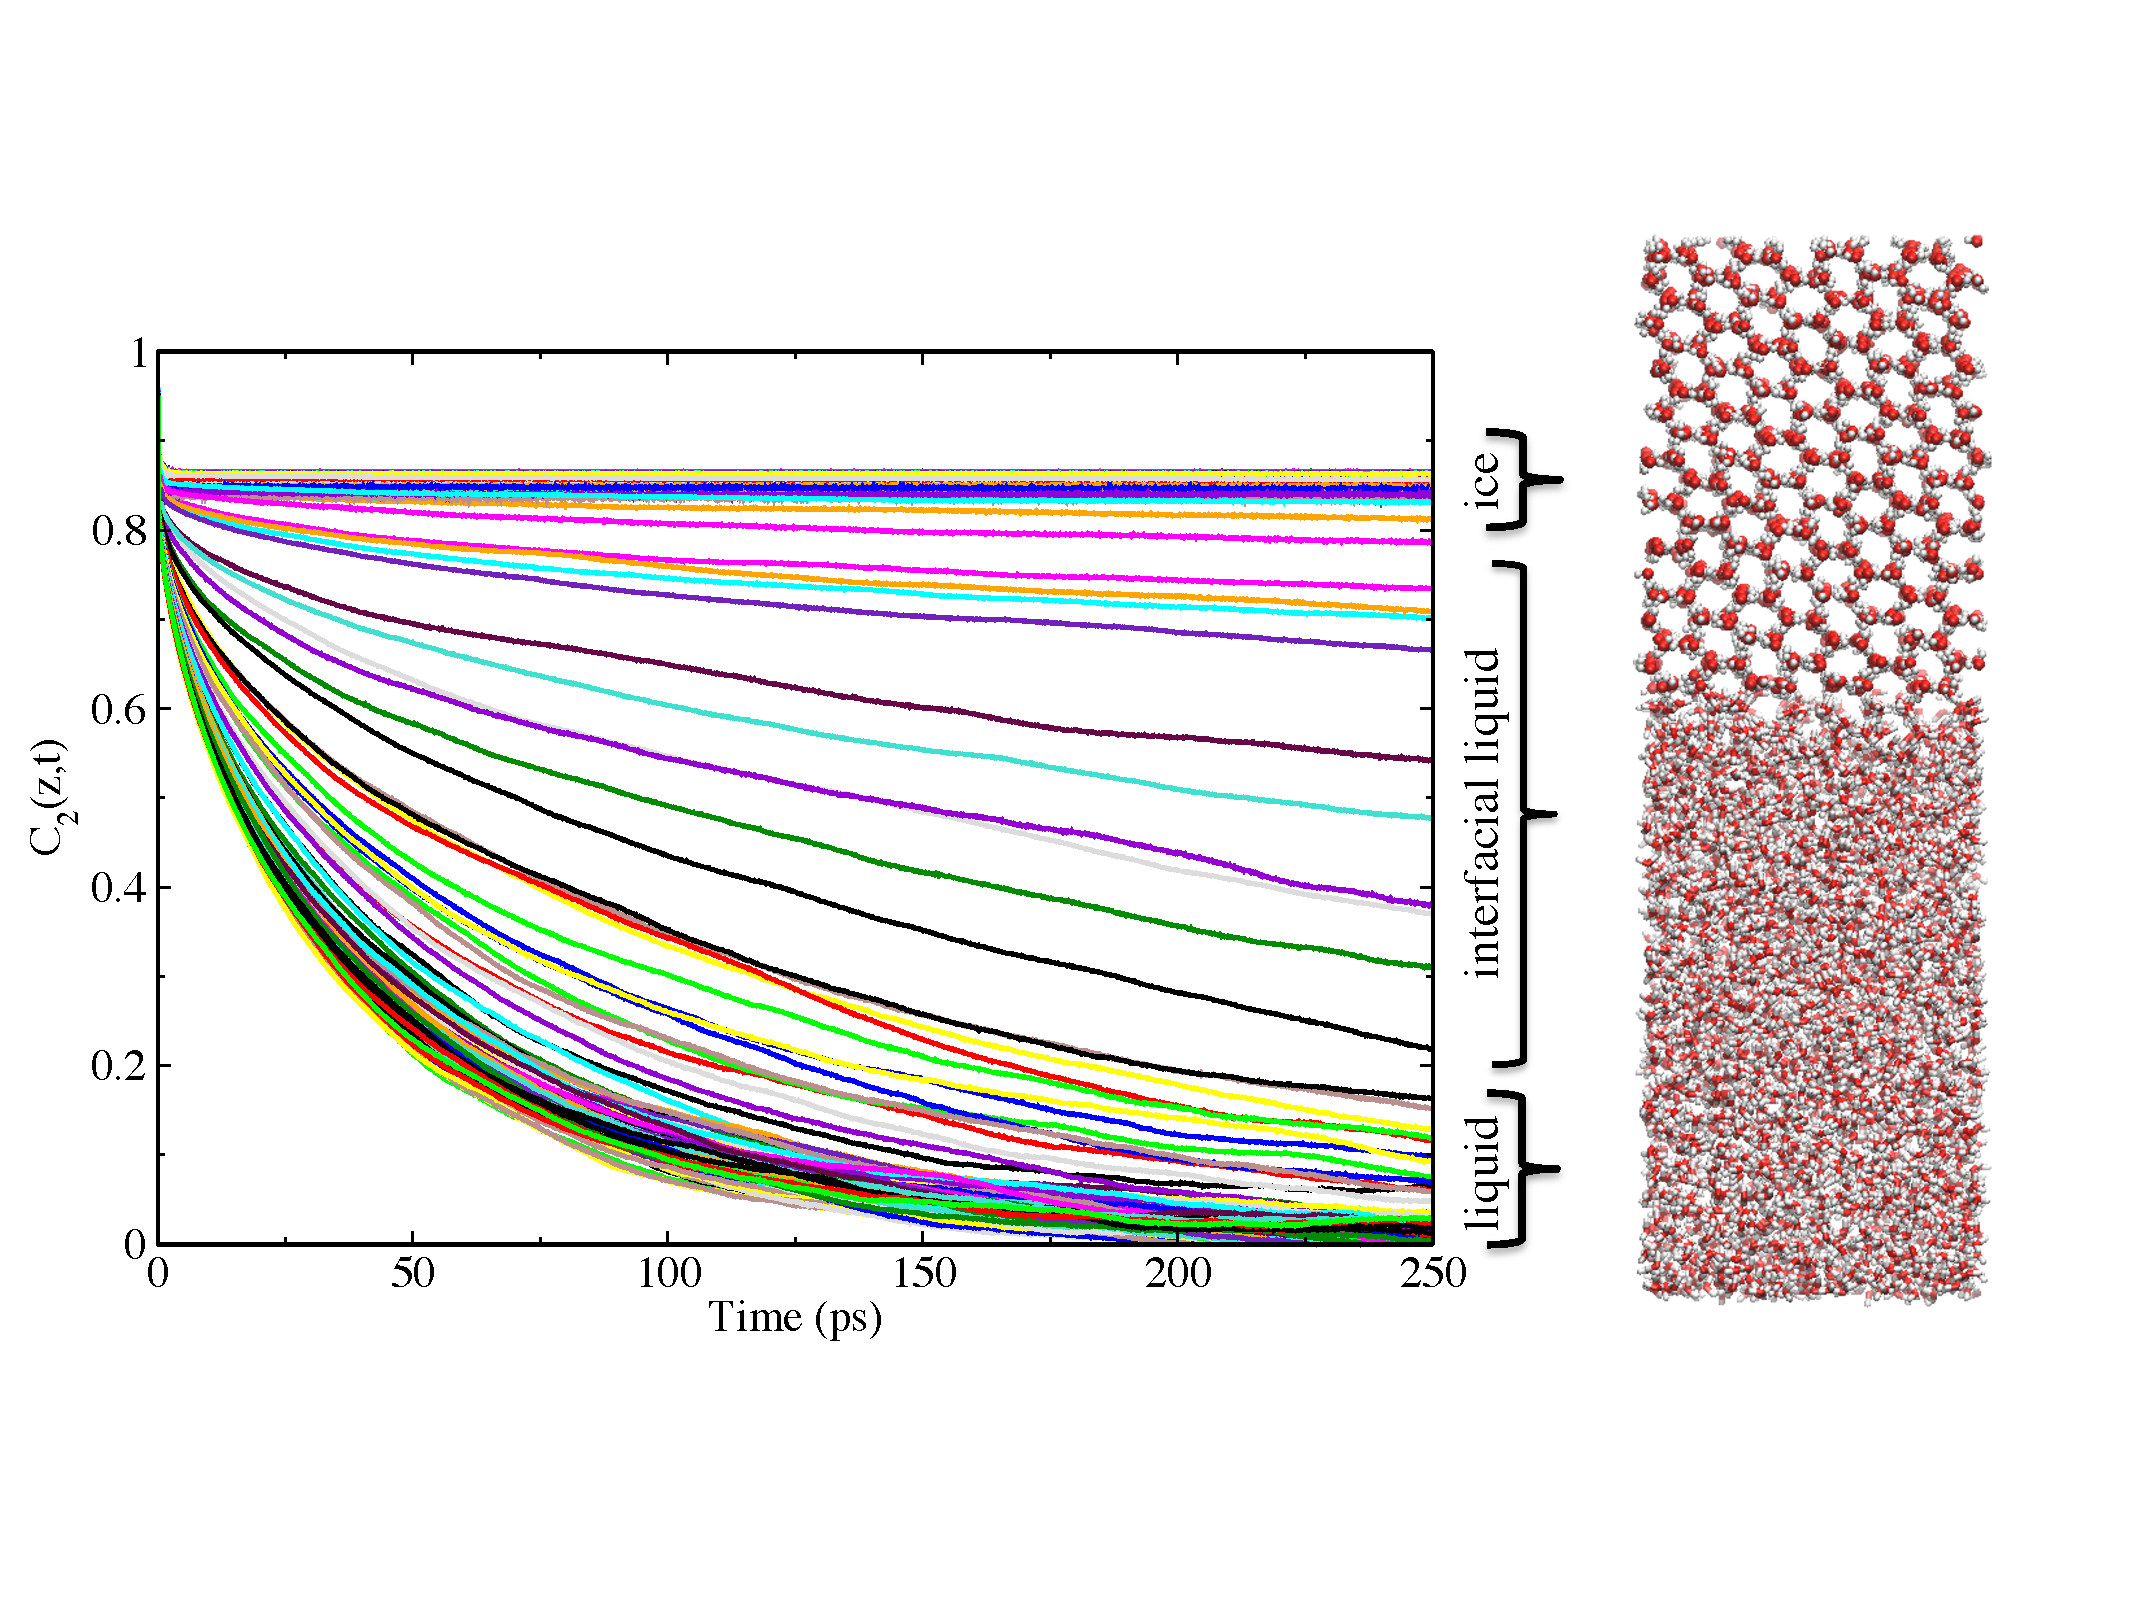
\includegraphics[width=\linewidth]{Figures/CztImage}
\caption{\label{fig:Czt} $C_2(z,t)$ collected in 1 \AA~bins across the SPC/E
  secondary prism ice / water interface. The band that experiences very
  little decay represents water molecules in the ice, while the band
  that decays quickly corresponds to bins in the liquid.  The
  correlation function presents a continuous distribution of decay
  behaviors across the interface between ice and liquid water.}
\end{figure}

Recently, Laage and Hynes have determined the mechanism for water
reorientation.\cite{Laage2006,Laage2008} Using molecular dynamics
simulations, they found that water reorients by breaking a hydrogen
bond with an overcoordinated first-shell neighbor, and makes a large
angle jump to form a new hydrogen bond with an undercoordinated
second-shell neighbor. The hydrogen bond cleavage and molecular
reorientation occur in a concerted fashion, not in successive steps as
was previously thought. With this detailed picture, they constructed
the Extended Jump Model\cite{Laage2006,Laage2008} based on the Ivanov
Jump Model and parameters extracted from their molecular simulations;
the average jump amplitude of the rotational jump, $\theta_{0}$, and
the frequency of the jumps, $1/\tau_{0}$. After accounting for
molecular frame reorientation, the Extended Jump Model is able to
predict reorientation relaxation times, $\tau_{n}^{jump}$, which agree
with experimental results as well as estimates obtained from
simulations where fast librational motion is ignored.

Computed $C_2(z,t)$ values have previously been fit to a
triexponential decay, with three time constants:
$\tau_\mathrm{short}$, measuring the librational motion of the water
molecules, $\tau_\mathrm{middle}$, measuring the timescale for the
large angle jumps during the breaking and making of hydrogen bonds,
and $\tau_\mathrm{long}$, corresponding to the translational motion of
the water molecules.\cite{Louden2013a} The Extended Jump Model also
includes three similar decay constants, however two of them are linked
and the dynamics of the decay is governed by two parameters. Since we
are interested in how the decay times and the individual contributions
may change through the interface, we have fit the $C_2(z,t)$ data
with
\begin{equation}
  C_{2}(z,t) = a~e^{-t/\tau_\mathrm{short}} + b~e^{-t/\tau_\mathrm{middle}} + 
  (1-a-b)~e^{-t/\tau_\mathrm{long}}
\label{eq:c2}
\end{equation}
where all of the decay constants are considered local functions of the
$z$ coordinate. In Fig. \ref{fig:SPorient}, the $z$-coordinate
profiles for the three decay constants, $\tau_{\mathrm{short}}$,
$\tau_{\mathrm{middle}}$, and $\tau_{\mathrm{long}}$ for the secondary prism interface
is shown, along with their fractional components of the overall total
decay, ($a$, $b$, $1-a-b$), respectively. Similar figures for the
other interfaces are provided in the Supporting Information.

In the liquid regions of all four interfaces, $\tau_\mathrm{middle}$
and $\tau_\mathrm{long}$ consistently approach $3-6$ ps and $30-40$
ps, respectively.  Both of these times increase closer to the
interface.  Conversely, $\tau_\mathrm{short}$ decreases from a
liquid-state value of $72-76$ fs approaching the interface.

The fractional contributions of the three motions to the overall decay
changes as we approach the interface as well. Far from the ice, the
librational motion and hydrogen bond breaking/making events each
contribute to about 20 percent of the total decay, whereas frame
reorientation contributes about 60 percent. As we approach the
interface, the librations and hydrogen bond dynamics both decrease in
contribution. The librations comprise approximately 15 percent of the
overall decay at the edge of the interface, whereas the hydrogen bond
contributions drop to approximately zero. In contrast, the fraction of
the total decay due to frame reorientation is shown to increase
approaching the interface.  The time constant corresponding to this
motion is seen to logarithmically increase as we approach the interface
as the molecules become more ice-like. In the ice we would expect
molecular reorientation to be incomplete, however, at the interface we
observe frame reorientation to contribute 85 percent of the overall
decay.

\newpage
\begin{figure}
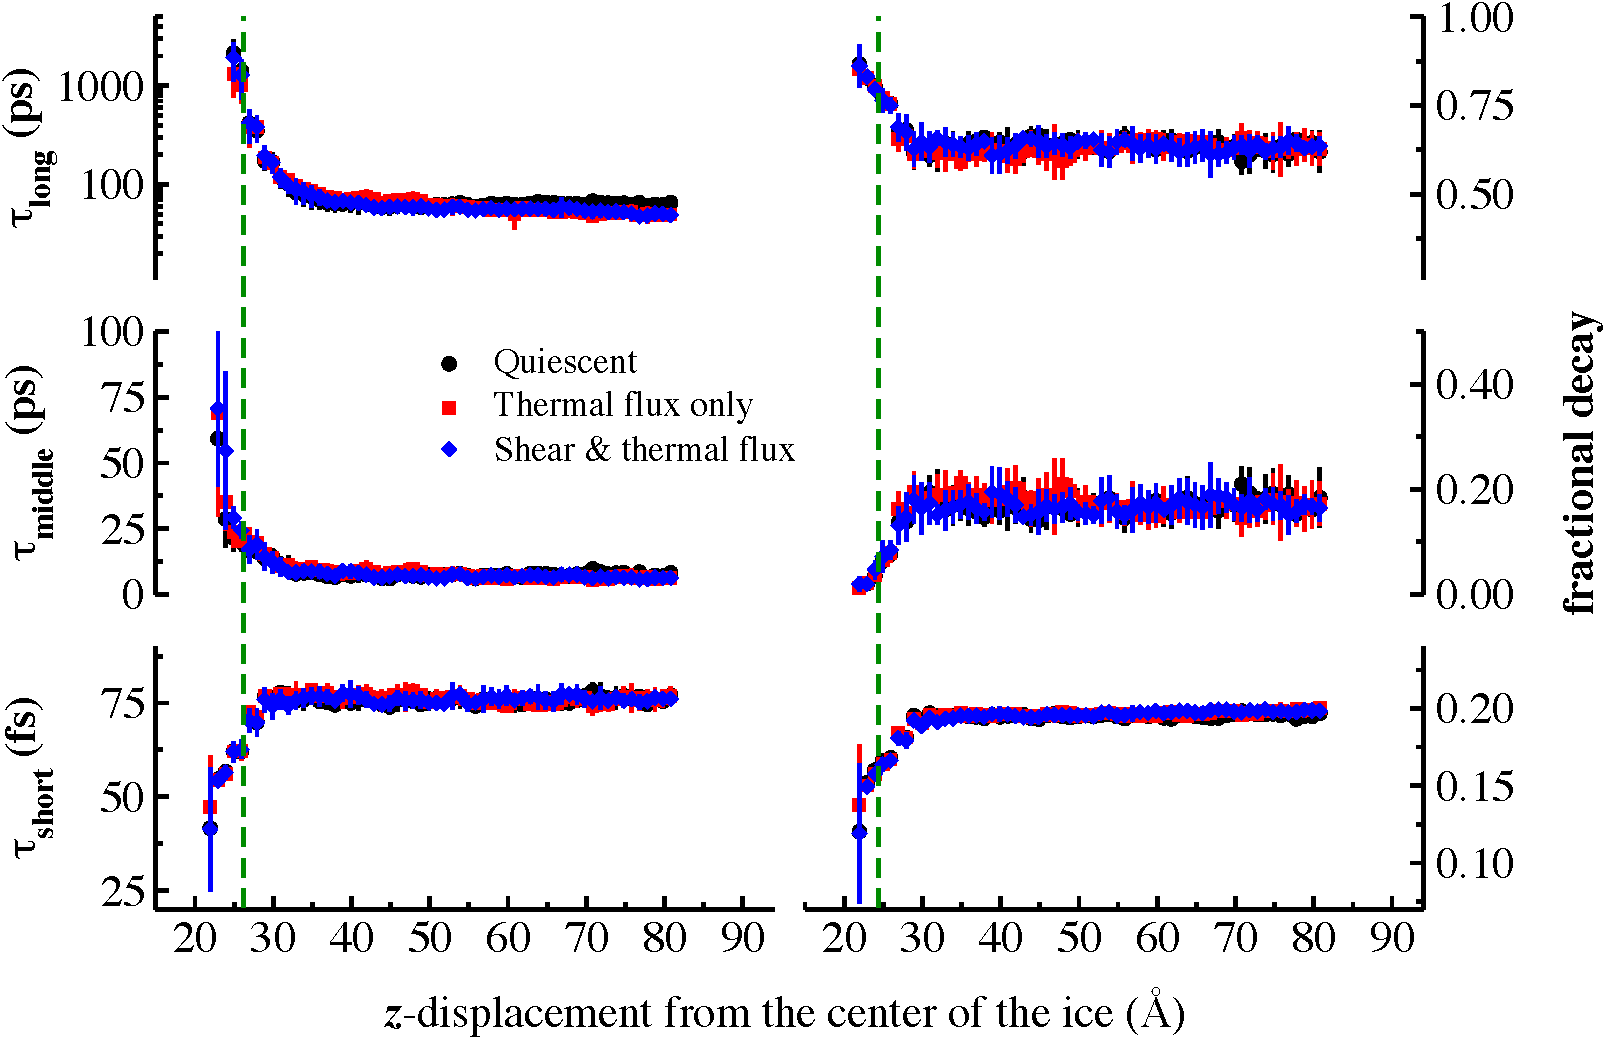
\includegraphics[width=\linewidth]{Figures/Sec_lcorrz}
\caption{\label{fig:SPorient} Decay times (left) for $C_2(z,t)$ at the
  SPC/E secondary prism interface, and their fractional contributions to the
  overall decay (right) fit using Eq. \eqref{eq:c2}. The local decay
  constants are plotted as a function of distance from the center of
  the ice slab. The vertical dashed line indicates the Gibbs dividing
  surface determined using the local tetrahedral order parameter.
  Results are shown for a quiescent system with no applied kinetic or
  momentum flux (black), an interface with an imposed
  kinetic energy flux (red), and a sheared simulation (blue) with both
  kinetic and momentum fluxes.}
\end{figure}

The middle and long decay times diverge inside the ice crystal, so the
orientational rate, $k(z) = 1 / \tau(z)$ can be used to identify a
dynamic interfacial width for the interface by fitting the profiles of
the middle and long-time orientational rates with a function that goes
smoothly between bulk-like liquid behavior and the crystal,
\begin{equation}\label{tauFit}
  k(z) = \frac{1}{\tau_\mathrm{liquid}} - \frac{1}{2~\tau_\mathrm{liquid}} \left(
      \tanh \left( \frac{z-l}{d} \right) - \tanh \left( \frac{z-r}{d} \right) \right)
\end{equation}
where $l$ and $r$ are the locations of the Gibbs dividing surfaces,
and $d$ is a dynamic width.  As with the structural widths,
$10\%-90\%$ dynamic widths are easily computed from the fits
($d_\mathrm{10-90} = 2.197~d$).  These values are provided in Tables
\ref{tab:propsSPCE} and \ref{tab:propsTIP4P}. All four SPC/E
interfaces exhibit dynamic widths that are $\sim 11$~\AA, and are
larger than the structural widths computed above.  In TIP4P/Ice at
270K, the dynamic widths are $\sim 14$~\AA, also larger than the
structural widths in for these interafaces.

We note that Bryk and Haymet also calculated the orientational time
correlation function at the basal interface of SPC/E
water,\cite{Bryk2002} and observed the same qualitative trend through
the ice / water interface, although the spatial resolution was not
sufficient to resolve a dynamic width.
 

\newpage   
\section{Orientational Decay Profiles}

\begin{figure}
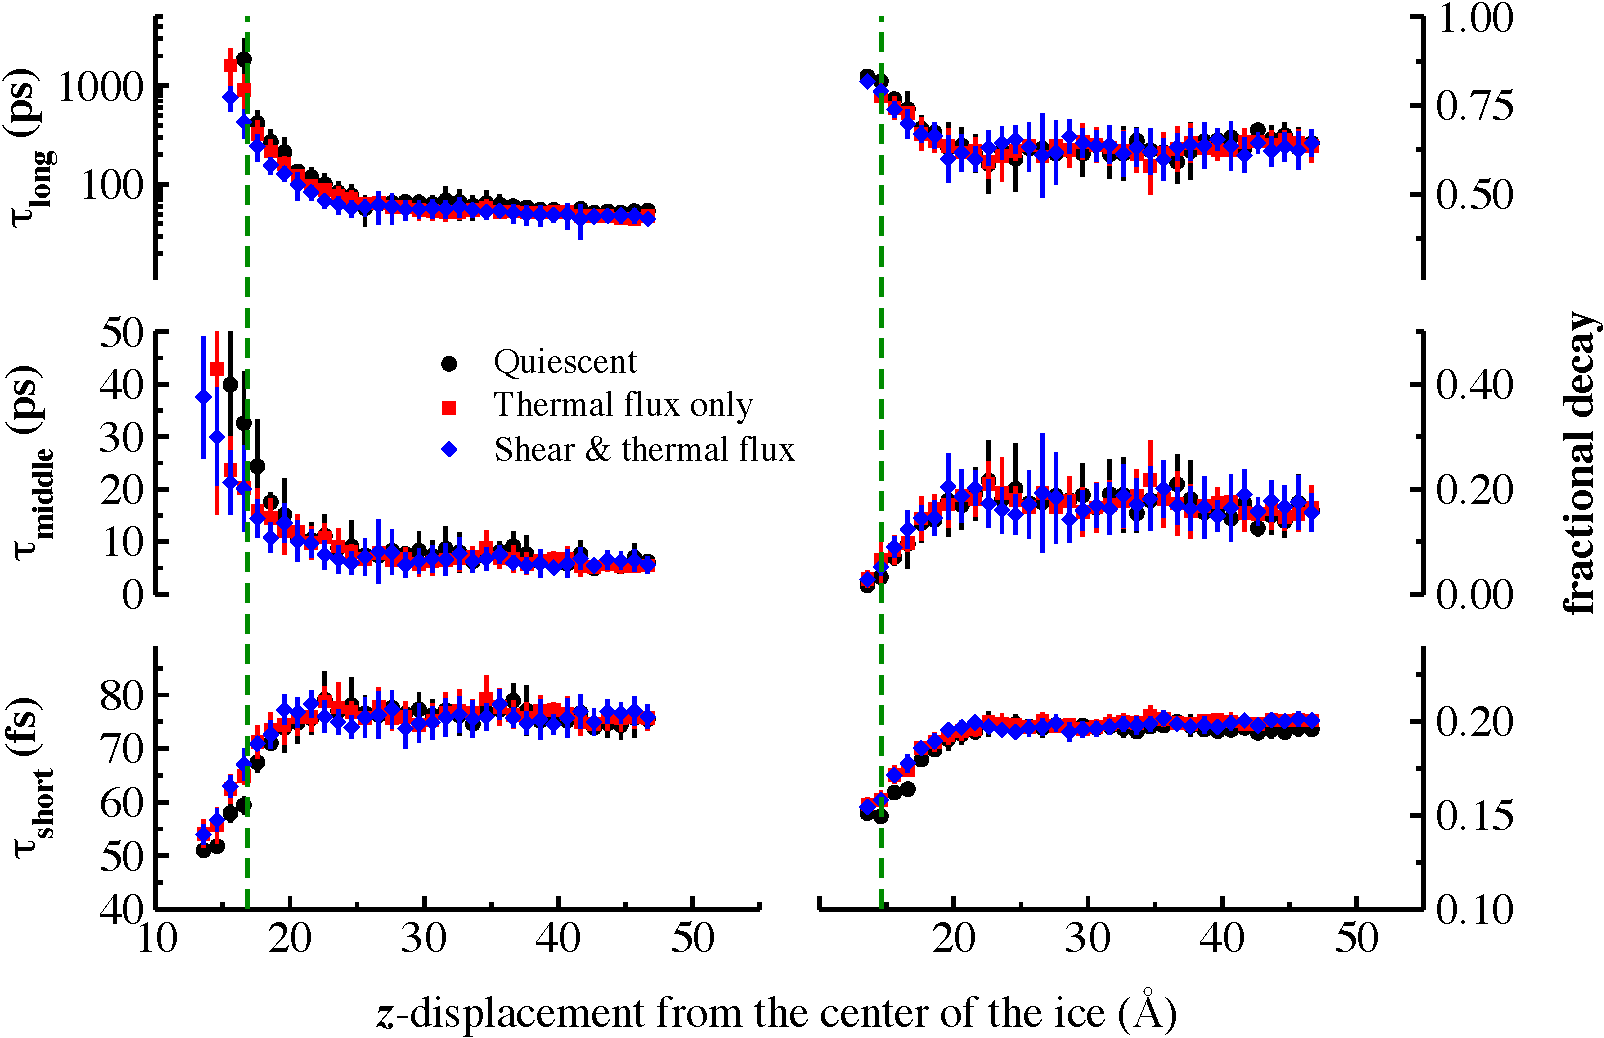
\includegraphics[width=\linewidth]{Figures/Pyr_lcorrz}
\caption{\label{fig:Pyrorient} Decay times (left) for $C_2(z,t)$ at
  the pyramidal interface, and their fractional contributions to the
  overall decay (right) fit using Eq. (8). The local decay constants
  are plotted as a function of distance from the center of the ice
  slab. The vertical dashed line indicates the Gibbs dividing surface
  determined using the local tetrahedral order parameter.  Results are
  shown for a quiescent system with no applied kinetic or momentum
  flux (black), an interface with with an imposed kinetic energy flux
  (red), and a sheared simulation (blue) with both kinetic and
  momentum fluxes.}
\end{figure}

\begin{figure}
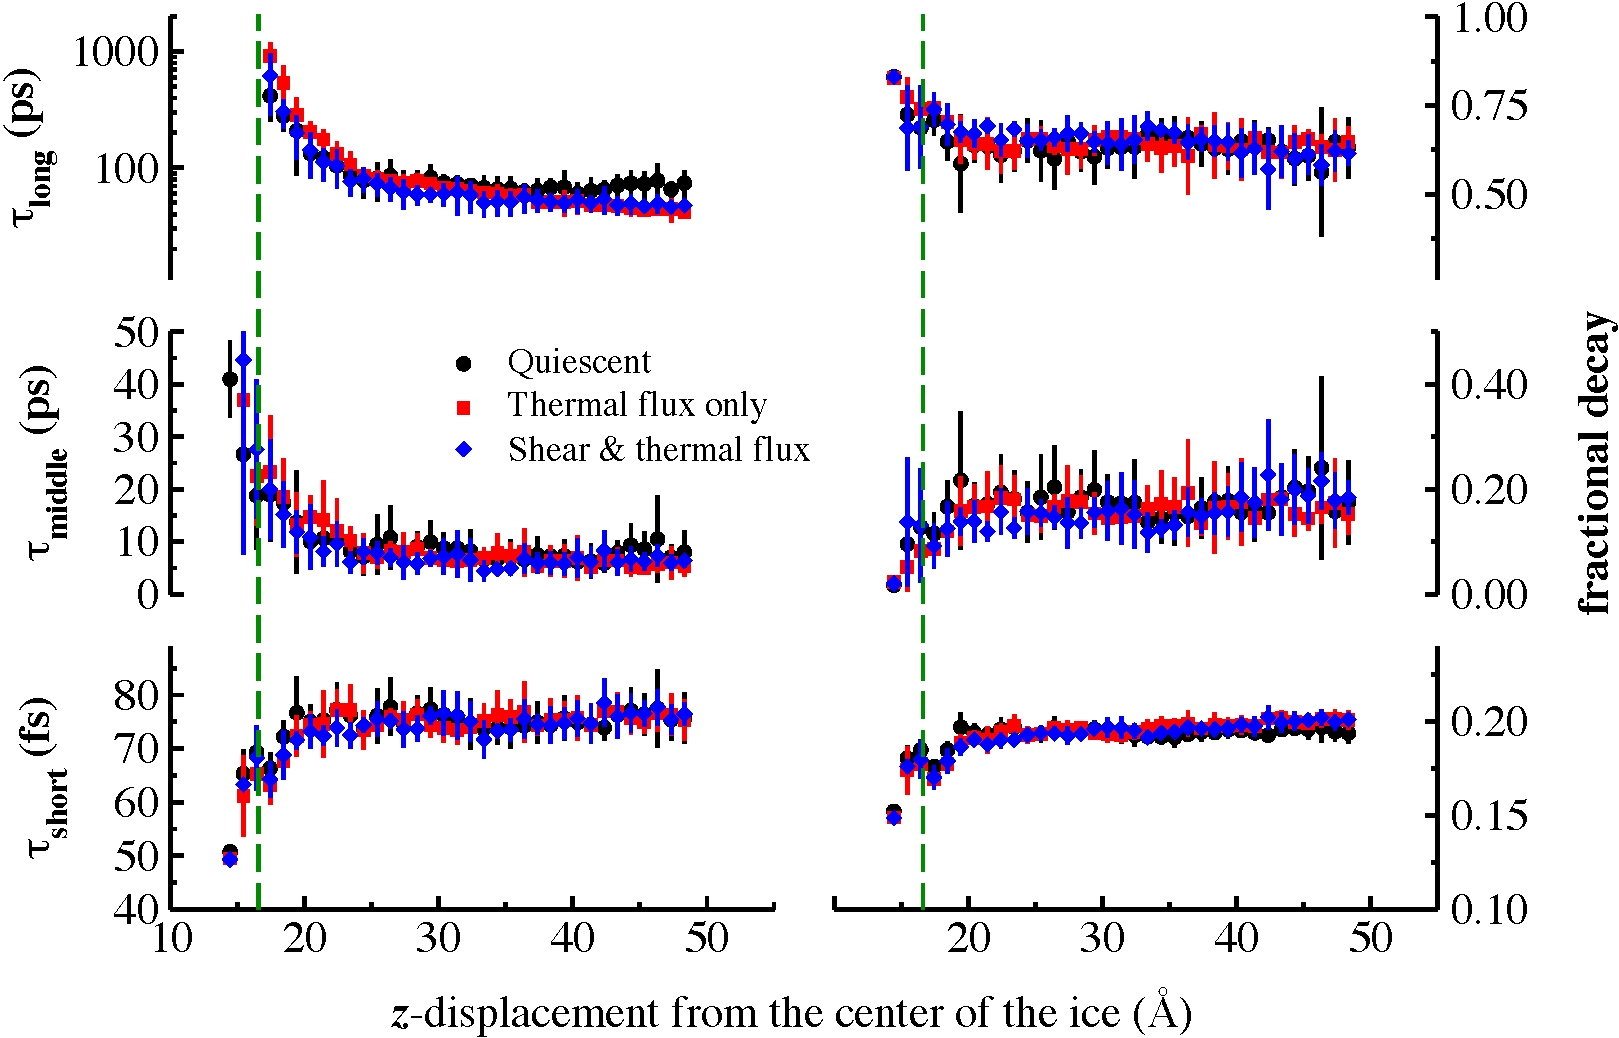
\includegraphics[width=\linewidth]{Figures/Bas_lcorrz}
\caption{\label{fig:Borient} $C_2(z,t)$ time constants for the basal
  interface.  Panel descriptions are the same as in
  Fig. \ref{fig:Pyrorient}. }
\end{figure}

\begin{figure}
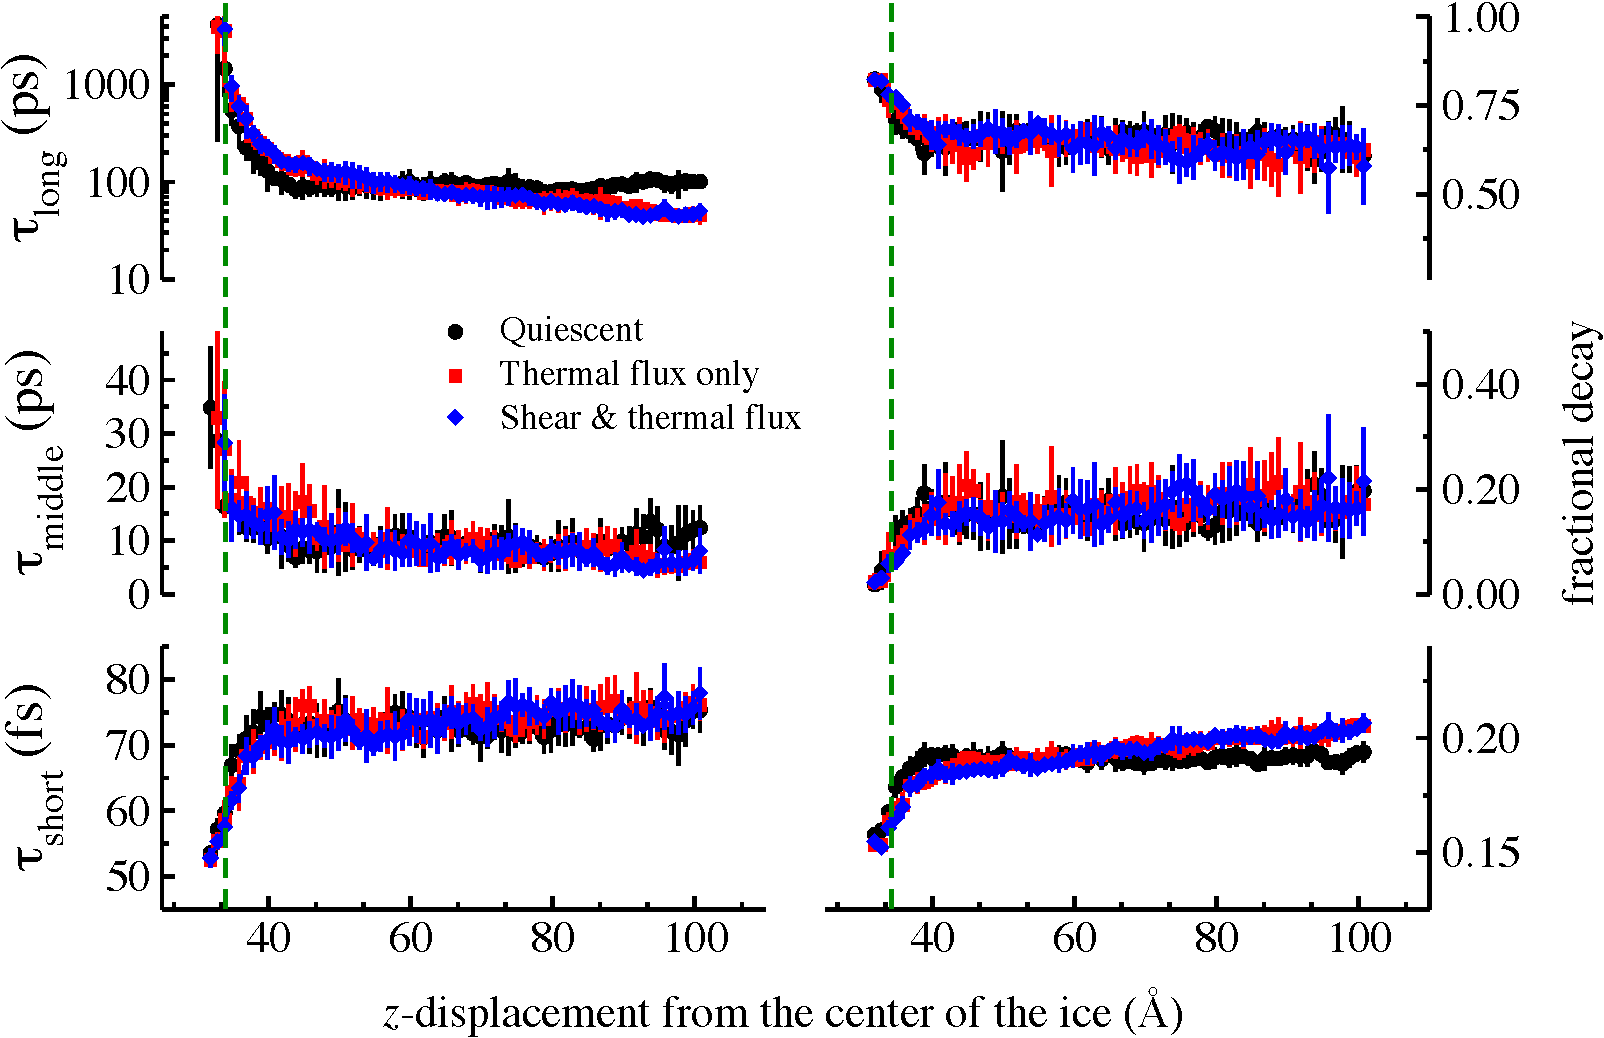
\includegraphics[width=\linewidth]{Figures/Pri_lcorrz}
\caption{\label{fig:Porient} $C_2(z,t)$ time constants for the prismatic
  interface.  Panel descriptions are the same as in
  Fig. \ref{fig:Pyrorient}.}
\end{figure}
%End z-orientation times       
